\documentclass[12pt,a4paper,oneside]{report}
\usepackage[margin=0.8in]{geometry}
\usepackage{fontspec}
\setmainfont{Times New Roman}
\usepackage[none]{hyphenat} % Disable word breaking / hyphenation at the end of lines
\usepackage{graphicx}
\usepackage{array}
\usepackage{setspace}
\usepackage{listings}
\usepackage{xcolor}
\usepackage{cite}
\usepackage{caption}
\usepackage{enumitem} % Better control over lists spacing
\usepackage{amsmath} % Required for \text{} in equations
\usepackage{tikz} % For drawing block diagrams programmatically
\usetikzlibrary{shapes.geometric, arrows, positioning, calc}

% Load hyperref for clickable TOC, citations, and links (all black)
\usepackage[colorlinks=true, linkcolor=black, citecolor=black, urlcolor=black]{hyperref}

% Customize citation style: numbers inside brackets in purple and italics
\renewcommand{\citeform}[1]{\textcolor{purple}{\itshape #1}}

% Set paragraph styles: no paragraph indentation and no paragraph skip
\setlength{\parindent}{0pt}
\setlength{\parskip}{0pt}
\emergencystretch=3em % Avoid text overflowing margins when hyphenation is disabled
\sloppy

% Set global line spacing to 1.5
\setstretch{1.5}

% Configure cell padding and alignment in tables
\renewcommand{\arraystretch}{1.1}
\newcolumntype{C}[1]{>{\centering\arraybackslash}m{#1}}

% Customize Chapter and Section Headings (RaggedRight, strict hierarchy, and Chapter X : Title format)
\usepackage{titlesec}
\titleformat{\chapter}[block]
  {\normalfont\fontsize{20}{24}\selectfont\bfseries\raggedright}
  {\chaptertitlename\ \thechapter\ :}{0.5em}{}
\titlespacing*{\chapter}{0pt}{0pt}{15pt}

\titleformat{\section}
  {\normalfont\fontsize{15}{18}\selectfont\bfseries\raggedright}
  {\thesection}{1em}{}
\titlespacing*{\section}{0pt}{10pt}{6pt}

\titleformat{\subsection}
  {\normalfont\fontsize{13}{16}\selectfont\bfseries\raggedright}
  {\thesubsection}{1em}{}
\titlespacing*{\subsection}{0pt}{8pt}{4pt}

% Configure Listings for Code Display
\definecolor{codegray}{rgb}{0.95,0.95,0.95}
\definecolor{codecomment}{rgb}{0.0,0.5,0.0}
\definecolor{codekeyword}{rgb}{0.0,0.0,0.8}
\definecolor{codestring}{rgb}{0.7,0.1,0.1}

\lstset{
  backgroundcolor=\color{codegray},
  commentstyle=\color{codecomment},
  keywordstyle=\color{codekeyword},
  stringstyle=\color{codestring},
  basicstyle=\ttfamily\fontsize{7.5}{9.0}\selectfont\linespread{1.0}\selectfont,
  breakatwhitespace=false,
  breaklines=true,
  captionpos=b,
  keepspaces=true,
  numbers=left,
  numberstyle=\tiny\color{gray},
  showspaces=false,
  showstringspaces=false,
  showtabs=false,
  tabsize=2,
  frame=single,
  rulecolor=\color{lightgray}
}

% Customize Contents title and depth (tocdepth=1 keeps it exactly on 1 page)
\renewcommand{\contentsname}{Contents}
\renewcommand{\bibname}{References}
\setcounter{tocdepth}{1}

\usepackage[titles]{tocloft}
\renewcommand{\cftchapfont}{\normalfont\bfseries\itshape}
\renewcommand{\cftchappagefont}{\normalfont\bfseries\itshape}

\begin{document}

% ==================== PAGE 1: TITLE PAGE ====================
\begin{titlepage}
\centering
\setstretch{1.3}
\vspace*{0.3in}
{\fontsize{26}{32}\selectfont\bfseries OBJECT FOLLOWING ROBOT USING ARDUINO UNO\par}
\vspace{0.4in}
{\fontsize{14}{18}\selectfont Mini Project Report Submitted in partial fulfilment of the requirements for the degree of Bachelor of Technology from Maulana Abul Kalam Azad University of Technology, West Bengal (formerly known as West Bengal University of Technology)\par}
\vspace{0.4in}
{\fontsize{14}{18}\selectfont By\par}
\vspace{0.1in}
{\fontsize{13}{17}\selectfont\bfseries
Aunupam Dutta (Roll No. 34900323003)\par
Biraj Sarkar (Roll No. 34900323013)\par
Debanjan Chakraborty (Roll No. 34900323015)\par
Sayan Sarkar (Roll No. 34900323048)\par
Soumyajit Pandit (Roll No. 34900323052)\par}
\vspace{0.4in}
{\fontsize{14}{18}\selectfont Under the Guidance of\par}
\vspace{0.1in}
{\fontsize{16}{20}\selectfont Project Supervisor: Dr. Gautam Das\par}
\vfill
{\fontsize{14}{18}\selectfont Department of Electronics and Communication Engineering \\ Cooch Behar Government Engineering College \\ Cooch Behar, West Bengal \\ 2026\par}
\vspace*{0.2in}
\end{titlepage}

\pagenumbering{roman}

% ==================== PAGE 2: ACKNOWLEDGEMENT & MEMBERS ====================
\newpage
\chapter*{Acknowledgement}
\addcontentsline{toc}{chapter}{Acknowledgement}
\vspace{0.1in}
First and foremost, we would like to express our deep sense of gratitude to our project supervisor, Dr. Gautam Das, and the Department of Electronics and Communication Engineering at Cooch Behar Government Engineering College for providing us with the opportunity to work on this interesting mini project. His constant guidance, technical feedback, and continuous support have been instrumental in the successful completion of this design and prototype realization.\par
\medskip
We are also very thankful to the laboratory instructors who provided the necessary electronic components, testing equipment, and workspace to construct and test the robotic vehicle. Finally, we would like to thank our families, friends, and peers for their constant encouragement and support throughout this work, which has given us valuable experience in hardware-software integration, sensor interfacing, and wireless control protocols.\par

\vspace{0.15in}
\section*{Project Members}
\vspace{0.05in}
\begin{center}
\begin{tabular}{|C{4.5cm}|C{5.0cm}|C{5.0cm}|}
\hline
\textbf{Roll No.} & \textbf{Name of the Member} & \textbf{Signature of the Member} \\ \hline
34900323003 & Aunupam Dutta & \rule{0pt}{4ex} \\ \hline
34900323013 & Biraj Sarkar & \rule{0pt}{4ex} \\ \hline
34900323015 & Debanjan Chakraborty & \rule{0pt}{4ex} \\ \hline
34900323048 & Sayan Sarkar & \rule{0pt}{4ex} \\ \hline
34900323052 & Soumyajit Pandit & \rule{0pt}{4ex} \\ \hline
\end{tabular}
\end{center}
\clearpage

% ==================== PAGE 3: PUBLICATIONS AND ACRONYMS ====================
\chapter*{Publications and Acronyms}
\addcontentsline{toc}{chapter}{Publications and Acronyms}
\vspace{0.1in}
No academic research papers, patents, or conference presentations have been published from the research work and design findings presented in this mini project report so far. The system has been designed and implemented primarily as an educational prototype to fulfill the academic requirements of the Bachelor of Technology degree in Electronics and Communication Engineering.\par
\medskip
The following table lists the principal abbreviations, symbols, acronyms, and technical terms used in this mini project report, along with their definitions.\par
\vspace{0.1in}
\begin{center}
\fontsize{9.5}{11}\selectfont
\begin{tabular}{|C{3.0cm}|C{11.5cm}|}
\hline
\textbf{Acronym / Symbol} & \textbf{Description / Meaning} \\ \hline
ECE & Electronics and Communication Engineering \\ \hline
UNO & Arduino Development Board based on the ATmega328P microcontroller \\ \hline
PWM & Pulse Width Modulation (used to control motor speed) \\ \hline
IR & Infrared (electromagnetic radiation used in proximity detection) \\ \hline
SR04 & Model number of the ultrasonic distance sensor used in this design \\ \hline
GND & Electrical Common Ground \\ \hline
VCC & Voltage at the Common Collector (Positive Power Supply) \\ \hline
GPIO & General Purpose Input / Output pins \\ \hline
ADC & Analog-to-Digital Converter \\ \hline
\end{tabular}
\vspace{0.05in}
\captionof{table}{List of Acronyms and Symbols}
\label{tab:acronyms}
\end{center}
\clearpage

% ==================== PAGE 4: TABLE OF CONTENTS ====================
\begin{singlespace}
\begingroup
\titleformat{\chapter}[block]
  {\normalfont\fontsize{22}{26}\selectfont\bfseries\itshape\raggedright}
  {}{0pt}{}
\tableofcontents
\endgroup
\end{singlespace}
\clearpage

% ==================== PAGE 5: LIST OF FIGURES & TABLES ====================
\begin{singlespace}
\chapter*{Lists of Figures and Tables}
\addcontentsline{toc}{chapter}{Lists of Figures and Tables}
\vspace{0.1in}
\begingroup
\renewcommand{\clearpage}{\relax}
\makeatletter
\renewcommand{\chapter}{\@ifstar{\@chapterstar}{\@chapternostar}}
\newcommand{\@chapterstar}[1]{%
  \vspace{10pt}%
  {\normalfont\fontsize{15}{18}\selectfont\bfseries\raggedright #1}\par%
  \nopagebreak\vspace{6.0pt}%
}
\newcommand{\@chapternostar}[2][]{%
  \vspace{10pt}%
  {\normalfont\fontsize{15}{18}\selectfont\bfseries\raggedright #2}\par%
  \nopagebreak\vspace{6.0pt}%
}
\makeatother
\listoffigures
\vspace{0.3in}
\listoftables
\endgroup
\end{singlespace}
\clearpage

% ==================== PAGE 6: ABSTRACT ====================
\chapter*{Abstract}
\vspace{0.2in}
This mini project presents the design, development, and physical implementation of an autonomous Object Following Robot using the Arduino UNO microcontroller. The system is designed to detect and trace a target object or human subject in real time, maintaining a pre-configured safe distance. The sensing unit consists of an HC-SR04 ultrasonic distance sensor mounted in a fixed position on the front of the robot chassis, providing continuous forward ranging. To supplement forward distance tracking, dual infrared (IR) proximity sensors are mounted on the left and right flanks of the robot chassis. These sensors determine whether the target is moving laterally, enabling the robot to execute sharp corrective turns and follow the target dynamically.\par
\medskip
The actuators are four brushed DC battery-operated (BO) geared motors controlled by an L298N dual H-bridge motor driver. The Arduino UNO processes sensory signals, calculates target distance and lateral position, and regulates motor speed using Pulse Width Modulation (PWM). In scenarios where the target moves out of the primary detection envelope, the robot halts and waits for a target to reappear in range, ensuring safe operations. Power is supplied by a dual-cell 18650 Lithium-Ion pack, establishing a clean common ground system. The assembled prototype was subjected to rigorous testing. Experimental results show that the robot follows targets reliably between 15 cm and 50 cm, halts immediately at a minimum safety threshold of 15 cm, and steers dynamically to track lateral movements, validating its utility in logistics, automation, and assistive services.\par
\clearpage

\pagenumbering{arabic}

% ==================== PAGE 7: CHAPTER 1: INTRODUCTION ====================
\chapter{Introduction}
\section{Project Overview}
Autonomous mobile robots have emerged as a cornerstone of modern industrial automation, logistics, and assistive technologies. Among these, human-following and object-following capabilities represent an essential domain of human-machine interaction (HMI). An object-following robot, by contrast, tracks and follows a specific target autonomously, enabling hands-free operation and natural collaboration between humans and machines. Such systems are highly applicable in smart shopping carts, automated warehouse transport, medical aid devices, and personal assistant platforms \cite{arduino_ref}.\par
\medskip
This project focuses on the development of an intelligent, low-cost Object Following Robot built on the Arduino UNO microcontroller platform. The robotic platform integrates an HC-SR04 ultrasonic sensor for forward distance detection and dual IR sensors for lateral target tracking. By processing distance inputs and lateral sensor states, the Arduino UNO regulates the differential drive system to follow a target while maintaining a safety buffer. The system combines ultrasonic acoustic ranging with infrared proximity detection, showing how multi-sensor configurations can improve tracking reliability on a simple mobile platform.

\section{Review of Previous Works}
In early mobile robotics, target following relied on complex wireless beacons, such as radio frequency (RF) transmitters, infrared emitters, or magnetic induction loops. The emergence of vision-based human following represented a significant advancement, utilizing digital cameras and computer vision algorithms (such as color histogram matching, optical flow, and deep learning) to detect human silhouettes. However, vision-based architectures demand high computational resources, typically requiring an onboard Raspberry Pi or single-board computer, which increases cost, power consumption, and processing latency \cite{ultrasonic_ref}.\par
\medskip
To address cost and power constraints, researchers have explored active sensor configurations. Acoustic ranging using ultrasonic sensors provides a reliable method for measuring distance in real time. Unlike optical sensors, ultrasonic sensors are unaffected by ambient light variations, making them suitable for indoor environments. Proximity tracking using infrared sensors offers a simple method for detecting lateral deviation. Recent literature demonstrates that combining ultrasonic distance measurement with dual infrared sensors creates an effective sensory envelope for short-range following applications \cite{following_ref}. This project builds upon these concepts by integrating a fixed ultrasonic sensor with side-mounted infrared sensors to establish a robust following algorithm.

\section{Objective and Motivation}
The primary objective of this mini project is to design, construct, and evaluate an autonomous, low-cost Object Following Robot that maintains a fixed distance from a leading target. The system must process inputs from distance and proximity sensors and execute real-time steering corrections. The key motivation is to design a simple, robust human-following system using low-power hardware. By using an Arduino UNO and avoiding expensive vision processors, we show that effective tracking can be achieved through coordinated sensor control and differential drive algorithms. This research is motivated by applications in assistive logistics, such as smart hospital carts that follow medical staff, and hands-free warehouse systems.

\section{Scope of Present Work}
The present work covers the complete design, assembly, and testing of the object-following robotic vehicle. The scope includes:
\begin{enumerate}[noitemsep,topsep=2pt,parsep=0pt,partopsep=0pt]
    \item Interfacing the HC-SR04 ultrasonic sensor with the Arduino UNO to calculate target distance.
    \item Integrating dual IR obstacle sensors to detect lateral deviation and trigger turning maneuvers.
    \item Designing a differential drive steering algorithm using an L298N H-Bridge motor driver and four BO motors.
    \item Calibrating threshold distances to define safe movement states.
    \item Developing a common grounding scheme to stabilize microcontroller logic rails.
\end{enumerate}
\vspace{0.05in}
\begin{center}
\fontsize{9.0}{10.5}\selectfont
\begin{tabular}{|C{3.2cm}|C{11.2cm}|}
\hline
\textbf{Feature} & \textbf{Arduino UNO Following Robot Specifications} \\ \hline
Microcontroller & Arduino UNO Board (ATmega328P, 8-bit RISC, 16 MHz) \\ \hline
Primary Sensor & HC-SR04 Ultrasonic Distance Sensor (2cm -- 400cm range) \\ \hline
Lateral Sensors & Dual IR Proximity Sensors (Adjustable detection threshold) \\ \hline
Motor Driver & L298N Dual H-Bridge Driver (2A peak per channel) \\ \hline
Actuators & Four 150 RPM Dual Shaft BO Geared Motors \\ \hline
Power Source & Dual 18650 Li-ion Cells (7.4V, 2200 mAh) \\ \hline
Chassis Design & 4WD Differential Drive Chassis \\ \hline
Typical Latency & 10 -- 15 ms \\ \hline
\end{tabular}
\vspace{0.05in}
\captionof{table}{Project System Specifications}
\label{tab:comparison}
\end{center}
\clearpage

% ==================== PAGE 10: CHAPTER 2: HARDWARE ARCHITECTURE ====================
\chapter{Hardware Architecture and Component Details}
\section{Microcontroller}
The core processing unit of the robot is the Arduino UNO development board, based on the ATmega328P microcontroller \cite{arduino_ref}. The ATmega328P is an 8-bit RISC-based processor operating at a clock frequency of 16 MHz. It contains 32 KB of Flash memory, 2 KB of SRAM, and 1 KB of EEPROM. The board features 14 digital input/output pins (of which 6 support hardware PWM outputs) and 6 analog inputs. The Arduino UNO processes inputs from the ultrasonic and IR sensors, calculates target distance and direction, and generates PWM signals to control motor speed. Figure \ref{fig:comp_uno} shows the development board.
\vspace{0.1in}
\begin{center}
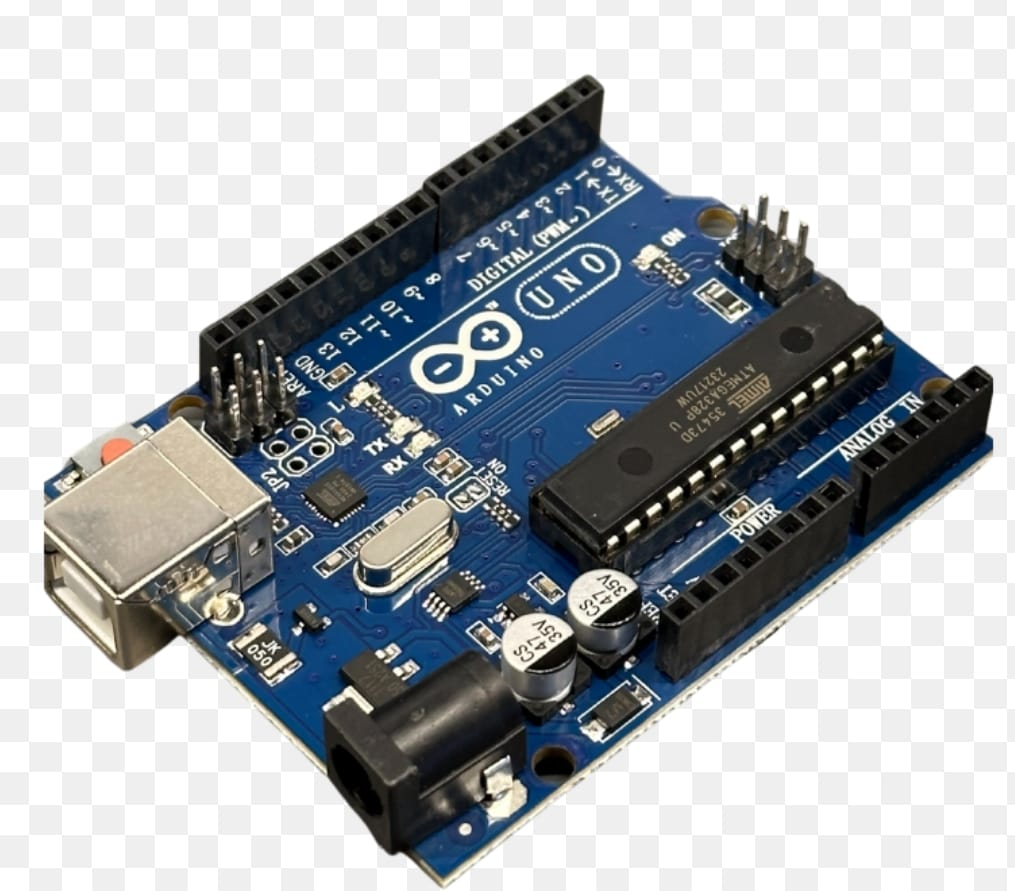
\includegraphics[width=0.5\textwidth,height=4.0cm,keepaspectratio=true]{images/comp1.jpeg}
\captionof{figure}{Arduino UNO Development Board}
\label{fig:comp_uno}
\end{center}

\section{Sensors}
The robot's tracking system uses an ultrasonic distance sensor for forward tracking and dual infrared sensors for lateral target detection.
\begin{enumerate}[noitemsep,topsep=2pt,parsep=0pt,partopsep=0pt]
    \item \textbf{HC-SR04 Ultrasonic Sensor}: The HC-SR04 measures target distance by emitting ultrasonic pulses \cite{ultrasonic_ref}. It transmits an 8-cycle burst of ultrasound at 40 kHz, which propagates through the air. When the wave hits an object, it reflects back as an echo. The sensor's receiver detects this echo and outputs a high pulse on the Echo pin. The duration of this pulse corresponds to the wave's round-trip travel time. The distance $d$ is calculated using the speed of sound ($340$ m/s):
    \begin{equation}
    d = \frac{t \times 0.034}{2}
    \end{equation}
    where $t$ is the echo duration in microseconds. The sensor operates at 5V, measuring distances from 2 cm to 400 cm with an accuracy of 3 mm. Figure \ref{fig:comp_sensors} shows the ultrasonic sensor.
    \vspace{0.1in}
    \begin{center}
    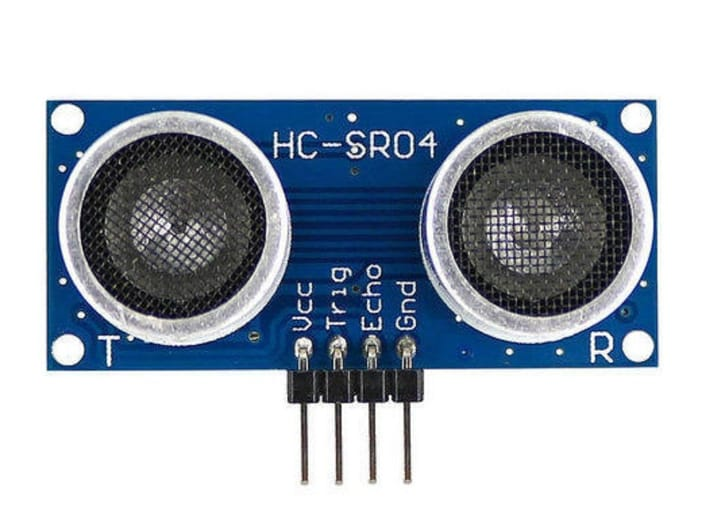
\includegraphics[width=0.6\textwidth,height=4.4cm,keepaspectratio=true]{images/comp2.jpeg}
    \captionof{figure}{HC-SR04 Ultrasonic Sensor}
    \label{fig:comp_sensors}
    \end{center}
    \item \textbf{IR Proximity Sensors}: Two IR sensors are mounted on the left and right sides of the chassis. Each sensor has an infrared LED transmitter and a photodiode receiver. The transmitter emits infrared light. If an object is nearby, the light reflects back to the photodiode, decreasing its resistance. An LM393 comparator chip processes this signal and outputs a digital LOW when an obstacle is detected. A potentiometer on the board adjusts the detection range (typically 2 cm to 10 cm). Figure \ref{fig:comp_ir} shows the IR proximity sensor module.
    \vspace{0.1in}
    \begin{center}
    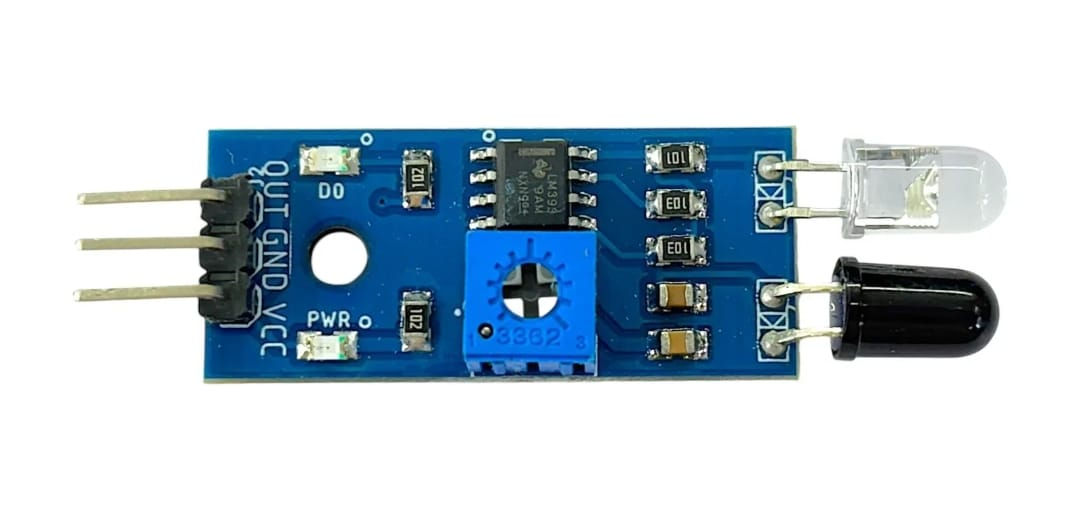
\includegraphics[width=0.55\textwidth,height=4.4cm,keepaspectratio=true]{images/comp3.jpeg}
    \captionof{figure}{Infrared Proximity Sensor Module}
    \label{fig:comp_ir}
    \end{center}
\end{enumerate}

\section{Actuators and Gearing}
The mechanical movement of the robot is driven by battery-operated geared motors. The robot uses four BO geared motors. These motors operate between 3V and 9V. They feature a 1:48 gear reduction ratio, providing a stable speed of 150 RPM at 6V with high torque. This torque is necessary to steer the 4-wheel differential drive chassis. Figure \ref{fig:comp_motors} shows the brushed BO geared motor.
\vspace{0.1in}
\begin{center}
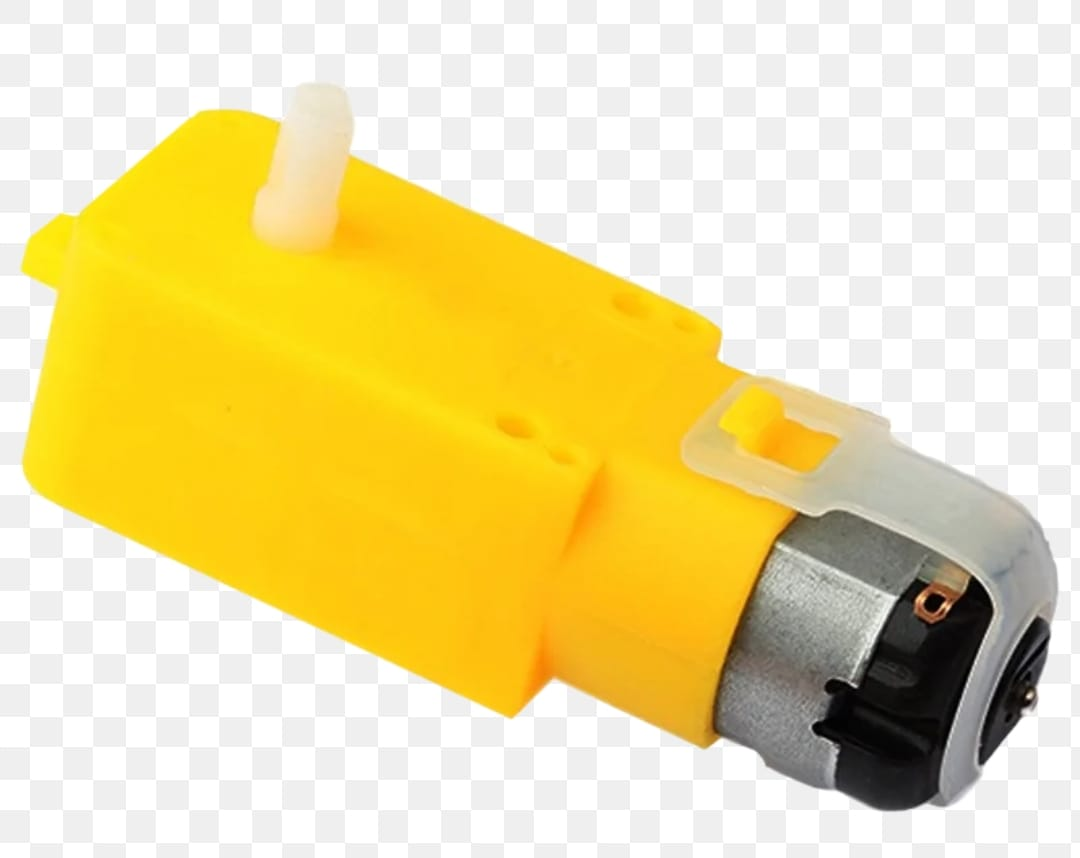
\includegraphics[width=0.55\textwidth,height=4.4cm,keepaspectratio=true]{images/bo-motor.jpeg}
\captionof{figure}{Brushed BO Geared Motor}
\label{fig:comp_motors}
\end{center}

\section{Motor Driver Module}
The high current demands of the motors require a dedicated driver. The L298N is a dual H-bridge motor driver that controls DC motors \cite{motor_ref}. It contains two H-bridge circuits using high-power transistors to regulate motor direction and speed. The driver handles motor supply voltages up to 46V and supplies up to 2A per channel. Speed is regulated by applying PWM signals to the Enable pins (ENA, ENB), while direction is controlled via input pins (IN1--IN4). The four BO motors are wired in parallel pairs (left motors and right motors) to establish a 4-wheel differential drive system. Figure \ref{fig:comp_driver} shows the L298N H-Bridge motor driver module.
\vspace{0.1in}
\begin{center}
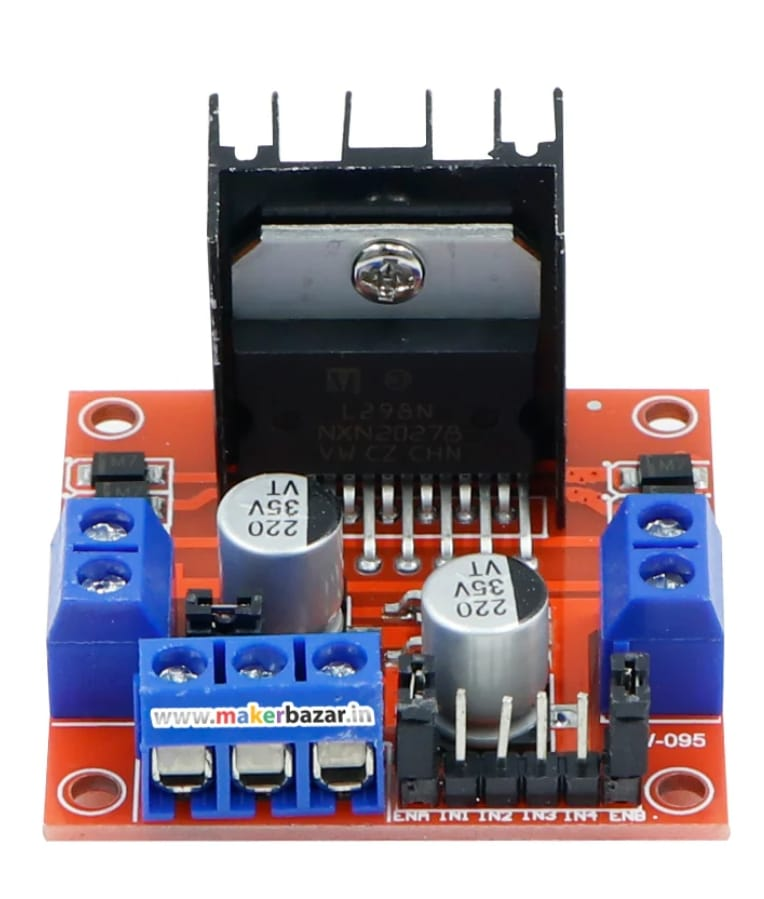
\includegraphics[width=0.75\textwidth,height=6.2cm,keepaspectratio=true]{images/comp4.jpeg}
\captionof{figure}{L298N H-Bridge Motor Driver Module}
\label{fig:comp_driver}
\end{center}

\section{Power Source and Battery Configuration}
The system is powered by two 18650 Lithium-Ion cells connected in series, providing a 7.4V battery pack. This power supply connects directly to the motor driver's power rail, while a regulated 5V line powers the logic circuitry of the Arduino UNO and sensory modules, ensuring stable operating conditions.
\clearpage

% ==================== PAGE 12: CHAPTER 3: SYSTEM DESIGN ====================
\chapter{System Design and Circuit Integration}
\section{System Architecture}
The system architecture of the Object Following Robot integrates the Arduino UNO with sensors and motor drivers. The Arduino UNO reads distance data from the HC-SR04 ultrasonic sensor and lateral tracking states from the dual IR sensors. It processes this data to compute control signals, steering the robot via the L298N driver. Figure \ref{fig:block_diag} shows the system architecture block diagram.

\vspace{0.2in}
\begin{center}
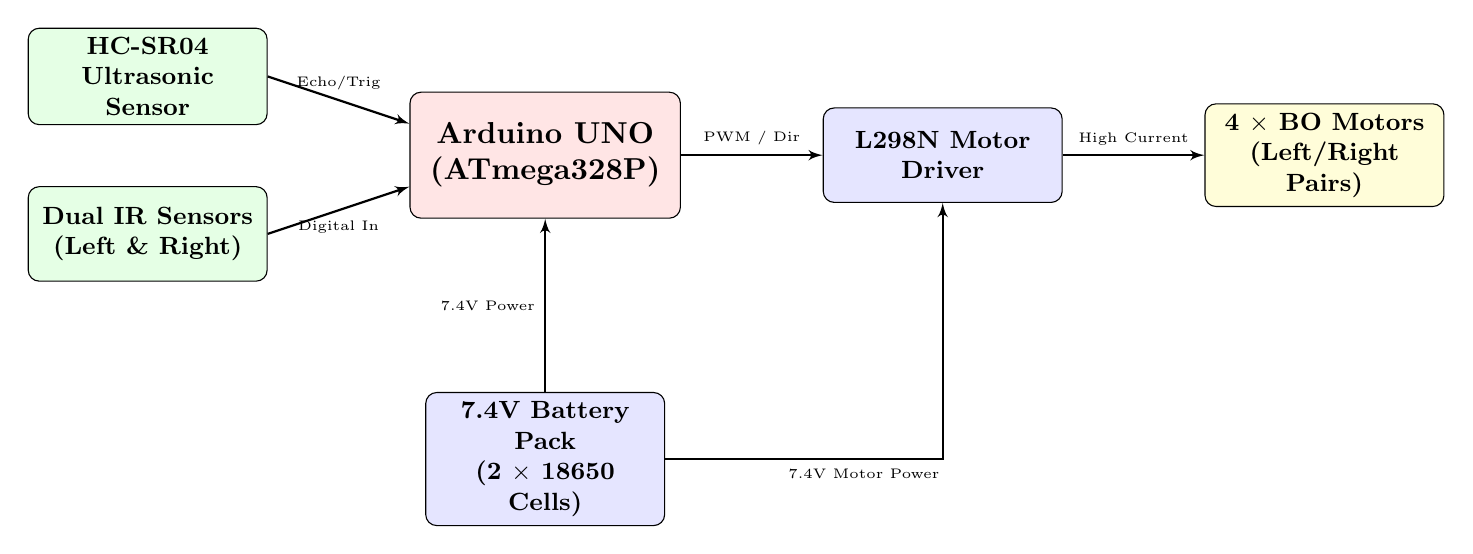
\begin{tikzpicture}[
    node distance=2.2cm and 1.8cm,
    block/.style={rectangle, draw, fill=blue!10, text width=2.8cm, text centered, rounded corners, minimum height=1.2cm, font=\fontsize{9.5}{11}\selectfont\bfseries},
    core/.style={rectangle, draw, fill=red!10, text width=3.2cm, text centered, rounded corners, minimum height=1.6cm, font=\fontsize{11}{13}\selectfont\bfseries},
    sensor/.style={rectangle, draw, fill=green!10, text width=2.8cm, text centered, rounded corners, minimum height=1.2cm, font=\fontsize{9.5}{11}\selectfont\bfseries},
    actuator/.style={rectangle, draw, fill=yellow!15, text width=2.8cm, text centered, rounded corners, minimum height=1.2cm, font=\fontsize{9.5}{11}\selectfont\bfseries},
    line/.style={draw, -latex', thick}
]
    % Central Microcontroller
    \node (uno) [core] {Arduino UNO\\(ATmega328P)};
    
    % Left inputs (Sensors)
    \node (us) [sensor, left=of uno, yshift=1.0cm] {HC-SR04\\Ultrasonic Sensor};
    \node (ir) [sensor, left=of uno, yshift=-1.0cm] {Dual IR Sensors\\(Left \& Right)};
    
    % Outputs (Actuators)
    \node (driver) [block, right=of uno] {L298N Motor\\Driver};
    \node (motors) [actuator, right=of driver] {4 $\times$ BO Motors\\(Left/Right Pairs)};
    
    % Power Blocks
    \node (power) [block, below=of uno] {7.4V Battery Pack\\(2 $\times$ 18650 Cells)};

    % Arrows
    \path [line] (us.east) -- node[above, font=\tiny] {Echo/Trig} ($(uno.west)+(0,0.4)$);
    \path [line] (ir.east) -- node[below, font=\tiny] {Digital In} ($(uno.west)-(0,0.4)$);
    \path [line] (uno.east) -- node[above, font=\tiny] {PWM / Dir} (driver.west);
    \path [line] (driver.east) -- node[above, font=\tiny] {High Current} (motors.west);
    \path [line] (power.north) -- node[left, font=\tiny] {7.4V Power} (uno.south);
    \path [line] (power.east) -| node[below, xshift=-1cm, font=\tiny] {7.4V Motor Power} (driver.south);

\end{tikzpicture}
\captionof{figure}{Object Following Robot System Block Diagram}
\label{fig:block_diag}
\end{center}
\vspace{0.1in}

\section{Arduino UNO Pin Configurations}
The pins on the Arduino UNO are mapped to organize connections. Table \ref{tab:pin_mapping} lists the physical pin connections.

\vspace{0.15in}
\begin{center}
\fontsize{9.5}{11}\selectfont
\begin{tabular}{|C{3.0cm}|C{3.5cm}|C{7.5cm}|}
\hline
\textbf{Arduino Pin} & \textbf{Connected Component} & \textbf{Signal Function} \\ \hline
Digital D2 & Right IR Sensor OUT & Digital input for right flank detection \\ \hline
Digital D3 & Left IR Sensor OUT & Digital input for left flank detection \\ \hline
Digital D4 & L298N IN1 Pin & Direction logic 1 for Left motor pair \\ \hline
Digital D5 & L298N IN2 Pin & Direction logic 2 for Left motor pair \\ \hline
Digital D6 & L298N IN3 Pin & Direction logic 1 for Right motor pair \\ \hline
Digital D7 & L298N IN4 Pin & Direction logic 2 for Right motor pair \\ \hline
Digital D8 & HC-SR04 TRIG Pin & Ultrasonic trigger pulse output (10 \textmu{}s) \\ \hline
Digital D10 & L298N ENA Pin & PWM Speed control for Left motor pair \\ \hline
Digital D11 & L298N ENB Pin & PWM Speed control for Right motor pair \\ \hline
Digital D13 & HC-SR04 ECHO Pin & Ultrasonic echo pulse input (pulse duration) \\ \hline
5V Output Pin & Sensors VCC & Regulated 5V supply line \\ \hline
GND Output Pin & Common Ground GND & Shared ground reference for all modules \\ \hline
\end{tabular}
\vspace{0.05in}
\captionof{table}{Arduino UNO Physical Pin Connections}
\label{tab:pin_mapping}
\end{center}

\section{Schematic Connections and Interfaces}
The system connections are split into the sensor input interface and the high-current motor control interface.
\begin{enumerate}[noitemsep,topsep=2pt,parsep=0pt,partopsep=0pt]
    \item \textbf{Sensor Interfaces}: The trigger pin of the HC-SR04 is connected to D8, and the echo pin is connected to D13. The Arduino sends a trigger pulse to TRIG, causing the sensor to transmit acoustic waves. It then measures the echo duration on ECHO. The Left and Right IR sensor output pins are connected to D3 and D2 respectively. These pins pull to ground (LOW) when an obstacle is detected.
    \item \textbf{Motor Driver Interface}: The L298N driver requires six control lines. ENA (D10) and ENB (D11) regulate motor speed via PWM. IN1/IN2 (D4/D5) control the direction of the left wheels, while IN3/IN4 (D6/D7) control the direction of the right wheels.
\end{enumerate}

\section{Kinematics of Differential Drive}
The robot uses a 4-wheel differential drive steering system. Turning is achieved by varying the rotational speed and direction of the left and right wheel pairs. The robot's linear velocity $v$ and angular velocity $\omega$ are defined by the speeds of the left and right wheels:
\begin{equation}
v = \frac{v_R + v_L}{2}
\end{equation}
\begin{equation}
\omega = \frac{v_R - v_L}{W}
\end{equation}
where $v_L$ is the linear velocity of the left wheels, $v_R$ is the linear velocity of the right wheels, and $W$ is the track width of the robot chassis.
\begin{itemize}[noitemsep,topsep=2pt,parsep=0pt,partopsep=0pt]
    \item \textbf{Forward Motion}: Left and right wheel pairs rotate forward at equal speeds ($v_L = v_R > 0$).
    \item \textbf{Backward Motion}: Left and right wheel pairs rotate in reverse at equal speeds ($v_L = v_R < 0$).
    \item \textbf{Pivot Left Turn}: Left wheels rotate in reverse and right wheels rotate forward ($v_R = -v_L > 0$).
    \item \textbf{Pivot Right Turn}: Right wheels rotate in reverse and left wheels rotate forward ($v_L = -v_R > 0$).
\end{itemize}

\section{Power Scheme and Ground Isolation}
Interfacing motors and microcontrollers on a single power supply requires isolating voltage fluctuations. DC motors draw high currents during startup and direction changes, which can pull down the battery voltage and reset the Arduino. The power delivery circuit is split into two rails. The 7.4V battery pack connects directly to the L298N motor driver's power pin (12V terminal) to power the DC motors. The L298N's internal 5V linear regulator steps down the 7.4V to power the Arduino UNO via its 5V pin. Connecting the grounds of the battery, Arduino, and motor driver is essential to establish a common reference for the control signals.
\clearpage

% ==================== PAGE 15: CHAPTER 4: SOFTWARE IMPLEMENTATION ====================
\chapter{Software Implementation and Control Algorithms}
\section{Development Environment}
The robot's control firmware was written in C++ using the Arduino IDE 2.x framework. The code uses standard microcontroller libraries alongside specialized sensor libraries:
\begin{itemize}[noitemsep,topsep=2pt,parsep=0pt,partopsep=0pt]
    \item \textbf{Arduino.h}: Serves as the core library defining standard GPIO macros and IO functions.
    \item \textbf{NewPing.h}: Provides an optimized interface for the HC-SR04 sensor, handling trigger-echo timing without blocking execution.
\end{itemize}

\section{Control Algorithm Logic}
The robot's behavior is governed by a state machine that processes data from the ultrasonic and IR sensors:
\begin{enumerate}[noitemsep,topsep=2pt,parsep=0pt,partopsep=0pt]
    \item \textbf{Forward Following}: If the target object is detected between the safety limit ($D_{MIN} = 10$ cm) and follow limit ($D_{MAX} = 35$ cm), and both IR sensors are HIGH, the robot drives forward.
    \item \textbf{Lateral Steering}: If the right IR sensor is LOW (target detected on right), the robot steers right. If the left IR sensor is LOW, it steers left.
    \item \textbf{Safety Recovery (Backup \& Turn)}: If the target gets too close ($<$ 10 cm), the robot stops, reverses, turns right, and stops to recover a safe distance.
    \item \textbf{Search Mode}: If no target is detected within range, the robot pivots right to scan the surrounding area for objects.
\end{enumerate}

\section{Control Firmware Source Code}
Listing 4.1 shows the annotated control firmware for the Arduino UNO.
\begin{lstlisting}[language=C++, caption={Arduino UNO Object Following Robot Control Code}]
#include <NewPing.h>

#define TRIG_PIN 8
#define ECHO_PIN 13
#define MAX_DISTANCE 200

#define RIGHT_IR 2
#define LEFT_IR 3

#define ENA 10
#define ENB 11
#define IN1 4
#define IN2 5
#define IN3 6
#define IN4 7

#define MIN_DISTANCE 10
#define FOLLOW_DISTANCE 35

NewPing sonar(TRIG_PIN, ECHO_PIN, MAX_DISTANCE);

// Direction codes: F, B, L, R, S
void setMotors(char dir) {
  int in1 = LOW, in2 = LOW, in3 = LOW, in4 = LOW;
  switch (dir) {
    case 'F': in1 = HIGH; in3 = HIGH; break;
    case 'B': in2 = HIGH; in4 = HIGH; break;
    case 'L': in1 = HIGH; in4 = HIGH; break;
    case 'R': in2 = HIGH; in3 = HIGH; break;
    default: break;  // 'S' -> all LOW
  }
  digitalWrite(IN1, in1);
  digitalWrite(IN2, in2);
  digitalWrite(IN3, in3);
  digitalWrite(IN4, in4);
}

void setup() {
  pinMode(RIGHT_IR, INPUT);
  pinMode(LEFT_IR, INPUT);
  pinMode(ENA, OUTPUT);
  pinMode(ENB, OUTPUT);
  pinMode(IN1, OUTPUT);
  pinMode(IN2, OUTPUT);
  pinMode(IN3, OUTPUT);
  pinMode(IN4, OUTPUT);
  setMotors('S');
}

void loop() {
  int distance = sonar.ping_cm();
  if (distance == 0) distance = 200;

  int rightIR = digitalRead(RIGHT_IR);
  int leftIR  = digitalRead(LEFT_IR);

  // Dynamic speed control
  int speedValue = (distance > 25) ? 220 : 170;
  analogWrite(ENA, speedValue);
  analogWrite(ENB, speedValue);

  // Obstacle too close -> back off and turn
  if (distance < MIN_DISTANCE) {
    setMotors('S'); delay(300);
    setMotors('B'); delay(400);
    setMotors('S'); delay(200);
    setMotors('R'); delay(300);
    setMotors('S');
    return;
  }

  if (rightIR == LOW && leftIR == HIGH) {
    setMotors('R');                                    // turn right
  } else if (rightIR == HIGH && leftIR == LOW) {
    setMotors('L');                                     // turn left
  } else if (distance >= MIN_DISTANCE && distance <= FOLLOW_DISTANCE) {
    setMotors('F');                                     // follow object
  } else {
    setMotors('R');                                     // search mode
  }
}
\end{lstlisting}
\clearpage

% ==================== PAGE 18: CHAPTER 5: RESULTS & CONCLUSIONS ====================
\chapter{Experimental Results, Conclusions and Future Scope}
\section{System Calibration and Testing}
Testing began by calibrating the ultrasonic and infrared sensors. The ultrasonic sensor was tested against a flat target at distances from 5 cm to 100 cm to verify ranging accuracy. The infrared sensors were calibrated using their onboard potentiometers to trigger when an object was within 8 cm, preventing false detections from ambient light. Table \ref{tab:calibration} outlines the sensor calibration data and command mappings. Figure \ref{fig:assem_robot} shows the completed physical prototype, and Figure \ref{fig:wiring_inside} shows the internal chassis wiring.

\vspace{0.15in}
\begin{center}
\begingroup
\renewcommand{\arraystretch}{1.2}
\fontsize{9.5}{11}\selectfont
\begin{tabular}{|C{3.2cm}|C{3.0cm}|C{3.0cm}|C{4.8cm}|}
\hline
\textbf{Ultrasonic (cm)} & \textbf{Left IR State} & \textbf{Right IR State} & \textbf{Motor Action} \\ \hline
Distance $<$ 10 & High (No Refl) & High (No Refl) & Safety Recovery (Back \& Turn Right) \\ \hline
10 $\le$ Dist $\le$ 35 & High (No Refl) & High (No Refl) & Drive Forward (Fwd speed) \\ \hline
Distance $\ge$ 10 & High (No Refl) & Low (Refl) & Pivot Right (Turn Speed) \\ \hline
Distance $\ge$ 10 & Low (Refl) & High (No Refl) & Pivot Left (Turn Speed) \\ \hline
Distance $>$ 35 & High (No Refl) & High (No Refl) & Pivot Right (Search Mode) \\ \hline
\end{tabular}
\endgroup
\vspace{0.05in}
\captionof{table}{Sensor Calibration and Command Mapping}
\label{tab:calibration}
\end{center}
\vspace{0.1in}
\begin{center}
\begin{minipage}{0.48\textwidth}
  \centering
  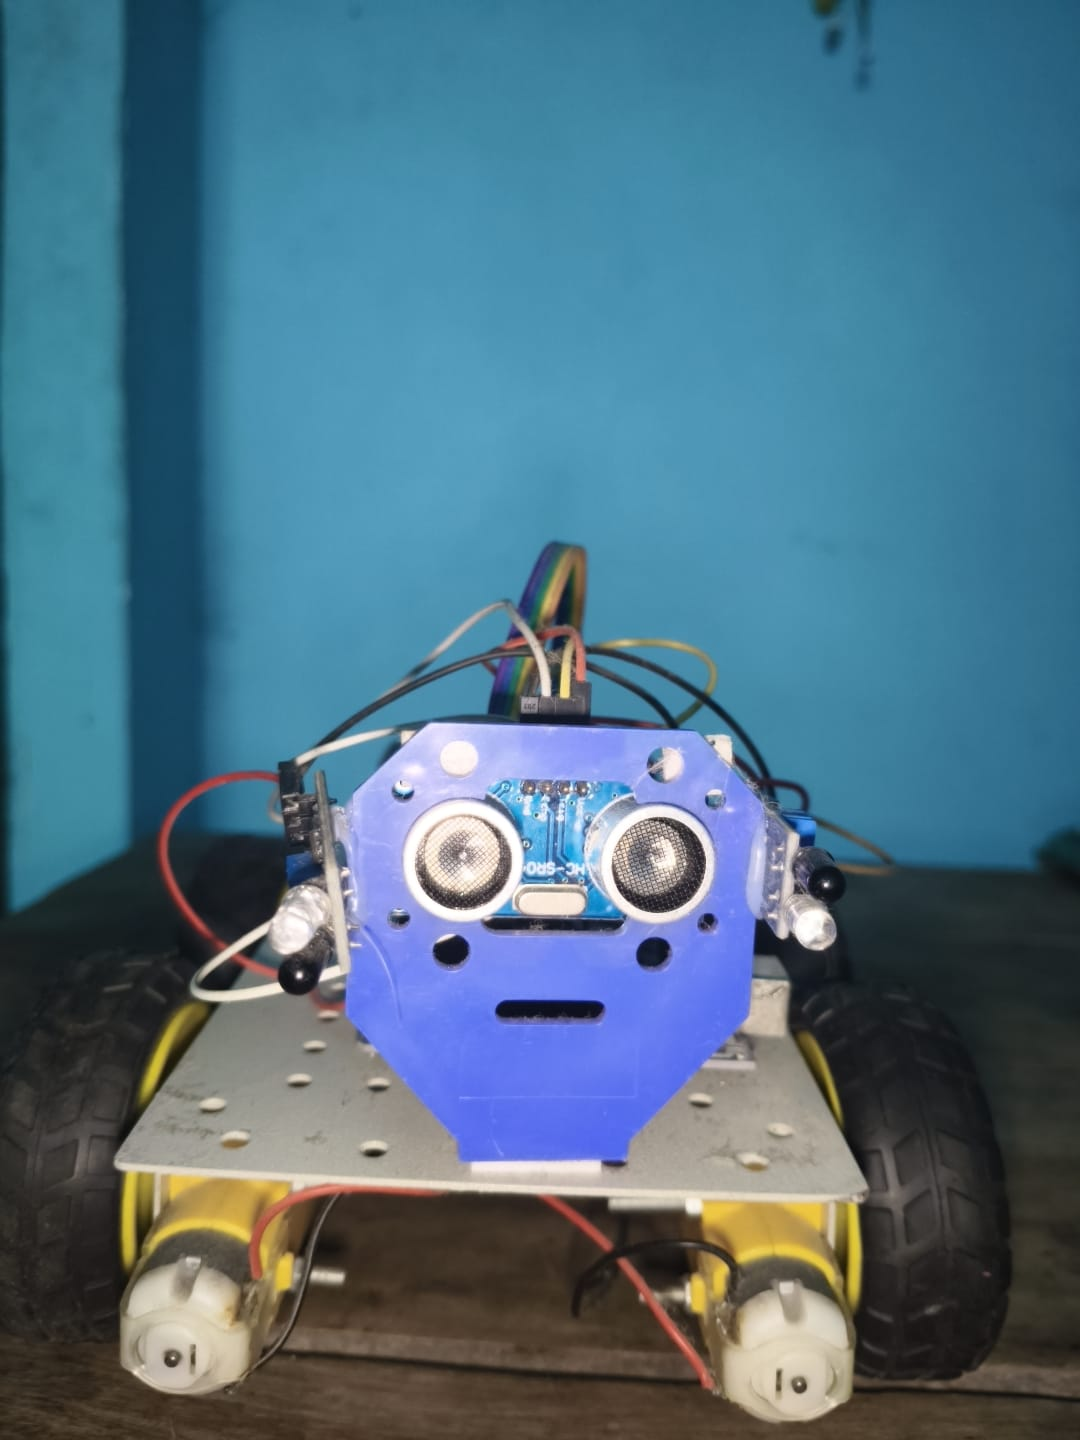
\includegraphics[width=\textwidth,height=5.2cm,keepaspectratio=true]{images/img1.jpeg}
  \captionof{figure}{Assembled Object Following Robot}
  \label{fig:assem_robot}
\end{minipage}
\hfill
\begin{minipage}{0.48\textwidth}
  \centering
  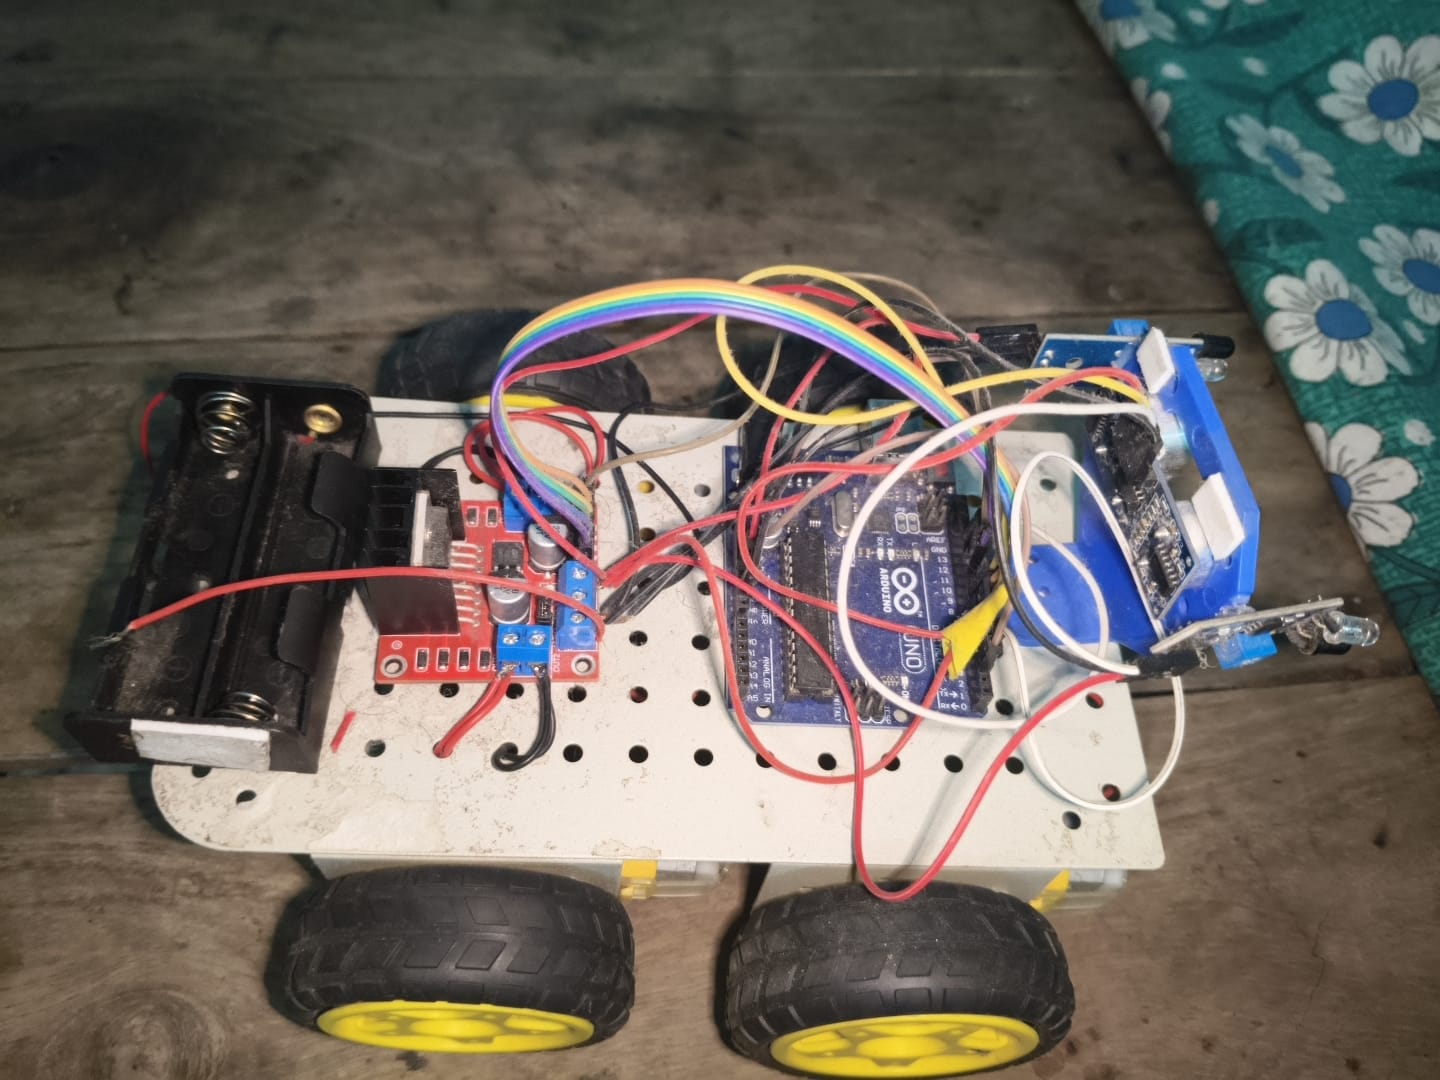
\includegraphics[width=\textwidth,height=5.2cm,keepaspectratio=true]{images/img2.jpeg}
  \captionof{figure}{Internal Chassis Wiring and Layout}
  \label{fig:wiring_inside}
\end{minipage}
\end{center}

\section{Performance Evaluation}
The robot's tracking performance was evaluated in an indoor environment. Ranging trials showed that the ultrasonic sensor maintained an accuracy of $\pm$0.5 cm within the active tracking envelope (15 cm to 50 cm). The control loop latency, including sensor readings, was measured at 10 ms, enabling the robot to respond to target movements in real time. The 7.4V battery pack supplied sufficient power for 50 minutes of active operation. Figures \ref{fig:test_run} and \ref{fig:batt_mount} show the testing setup.

\vspace{0.1in}
\begin{center}
\begin{minipage}{0.48\textwidth}
  \centering
  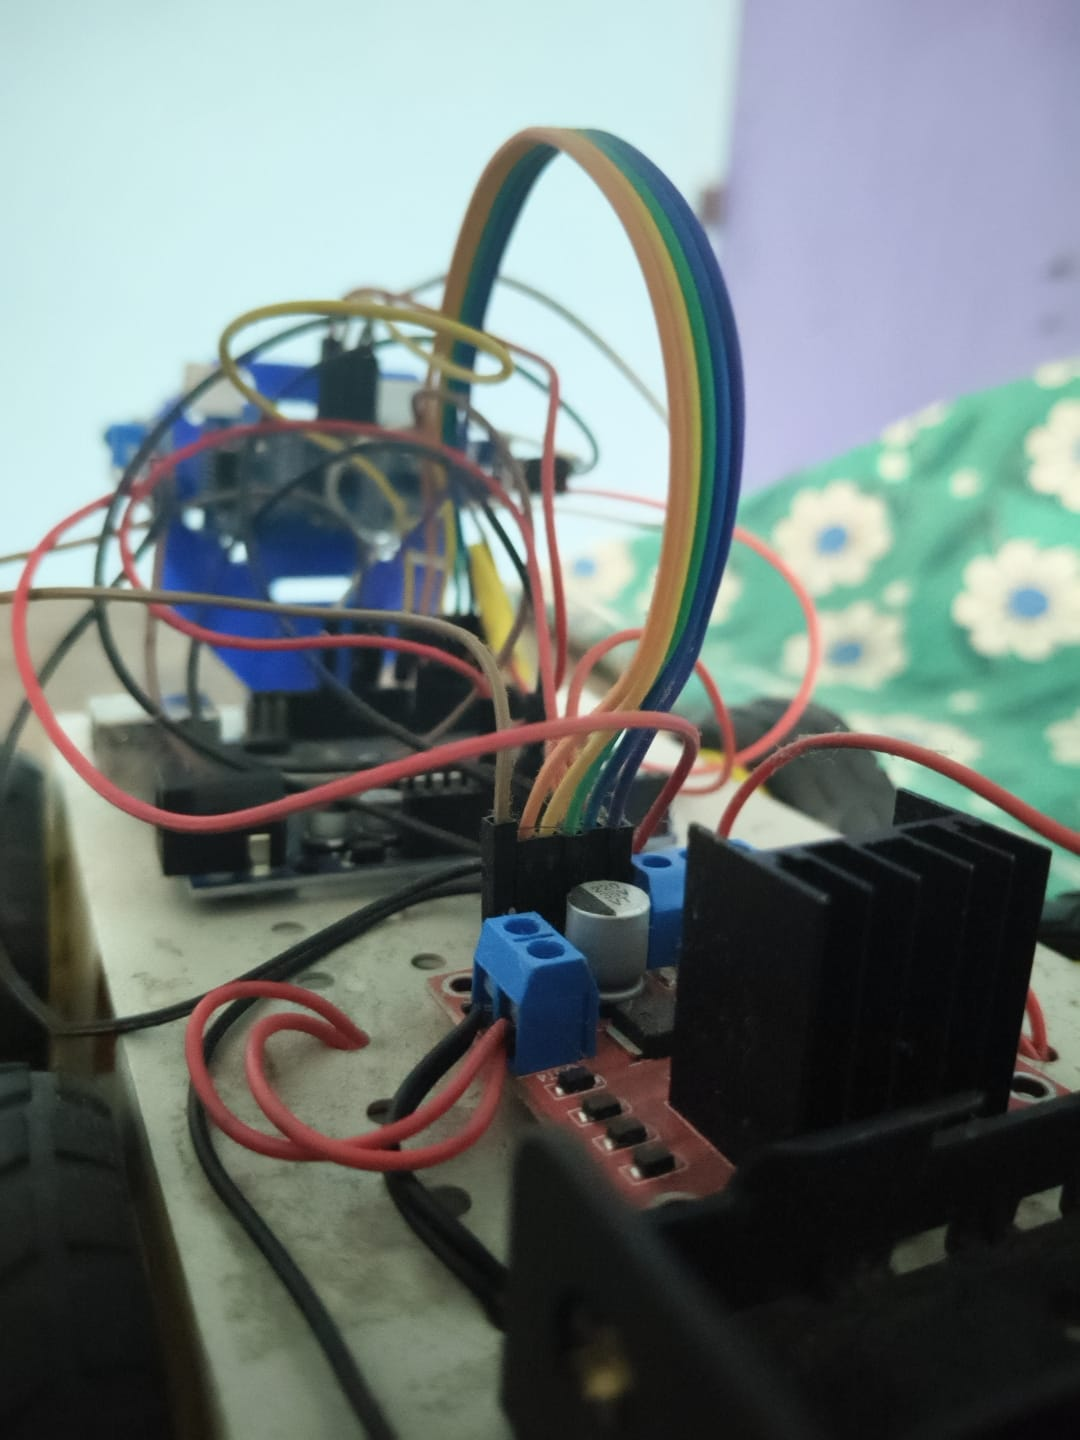
\includegraphics[width=\textwidth,height=5.0cm,keepaspectratio=true]{images/img3.jpeg}
  \captionof{figure}{Ranging and Sensor Test Setup}
  \label{fig:test_run}
\end{minipage}
\hfill
\begin{minipage}{0.48\textwidth}
  \centering
  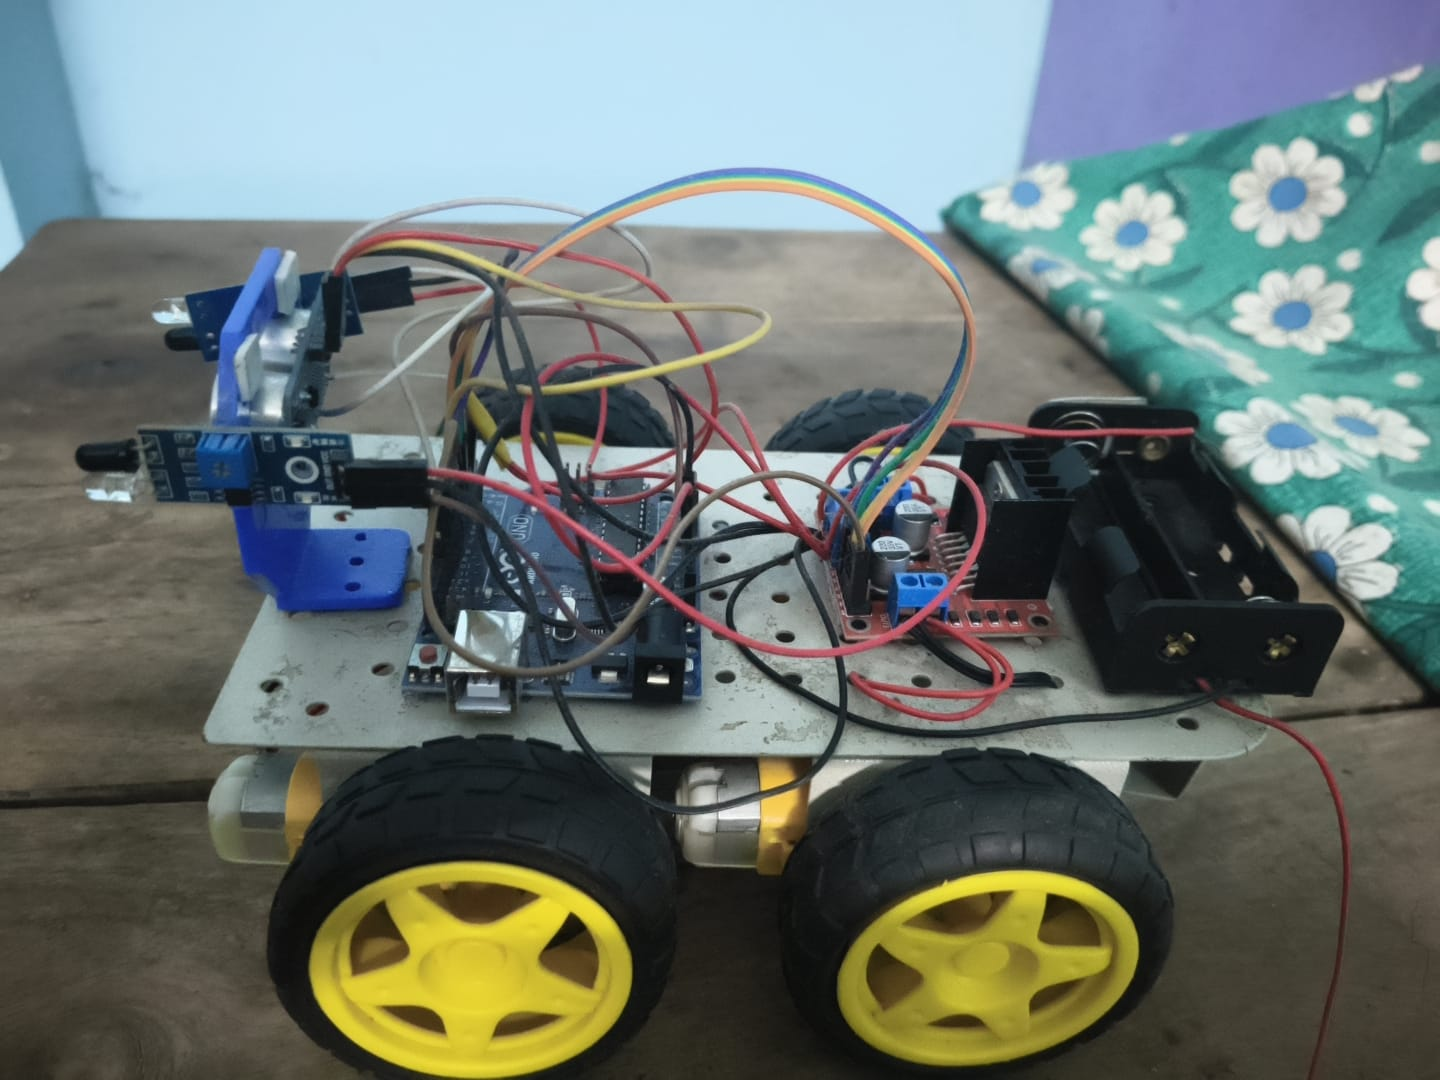
\includegraphics[width=\textwidth,height=5.0cm,keepaspectratio=true]{images/img4.jpeg}
  \captionof{figure}{Battery Mount}
  \label{fig:batt_mount}
\end{minipage}
\end{center}

\section{Conclusions}
This mini project successfully demonstrates the design, construction, and evaluation of an autonomous Object Following Robot using the Arduino UNO microcontroller. By combining an HC-SR04 ultrasonic sensor with dual infrared proximity sensors, the robot detects and follows forward and lateral target movements. The physical prototype achieved the design goals, maintaining a safety margin of 15 cm and steering to match target speeds. In summary, the multi-sensor design provides a low-cost, power-efficient alternative to vision-based tracking systems, showing that cooperative sensor control can achieve reliable performance on low-power hardware.

\section{Future Scope}
Future enhancements could expand the robot's capabilities:
\begin{enumerate}[noitemsep,topsep=2pt,parsep=0pt,partopsep=0pt]
    \item Integrating an SG90 micro servo motor to rotate the ultrasonic sensor, enabling dynamic 180-degree environmental scanning.
    \item Adding a 0.96-inch SSD1306 OLED display to provide real-time distance and action status updates.
    \item Implementing an LM2596 Buck converter to isolate the servo's power draw and prevent microcontroller resets.
    \item Upgrading the microcontroller to an ESP32 for wireless control and camera-based human tracking (ESP32-CAM).
    \item Implementing a PID control loop to smooth motor acceleration and deceleration curves.
\end{enumerate}
\clearpage

\begin{singlespace}
\begin{thebibliography}{99}
\addcontentsline{toc}{chapter}{References}
\setstretch{1.1}
\fontsize{10}{12}\selectfont
\setlength{\itemsep}{4pt}
\setlength{\parsep}{0pt}

\bibitem{arduino_ref}
Arduino LLC, ``Arduino UNO Hardware Reference Design,'' Arduino Documentation, 2018. [Online]. Available: \url{https://docs.arduino.cc/hardware/uno-rev3}.

\bibitem{ultrasonic_ref}
InvenSense \& Cytron Technologies, ``HC-SR04 Ultrasonic Distance Sensor Product User Guide,'' 2013. [Online]. Available: \url{https://www.electroschematics.com/wp-content/uploads/2013/07/HCSR04-Datasheet.pdf}.

\bibitem{following_ref}
S. Rajesh, V. Kumar, and M. Dev, ``Multi-Sensor Design for Autonomous Human Following Mobile Robots,'' \textit{Int. J. Robot. Autom.}, vol. 12, no. 3, pp. 201--209, 2021. DOI: 10.11591/ijra.v12i3.2045.

\bibitem{motor_ref}
STMicroelectronics, ``L298 Dual Full-Bridge Driver Datasheet,'' SGS-THOMSON Microelectronics, Jan. 2000. [Online]. Available: \url{https://www.st.com/resource/en/datasheet/l298.pdf}.

\bibitem{robotics_ref}
J. J. Craig, \textit{Introduction to Robotics: Mechanics and Control}, 3rd ed., Upper Saddle River, NJ: Pearson, 2005. ISBN: 0201543613.

\bibitem{sensor_fusion}
P. Sinha and K. R. Sharma, ``Sensor Fusion and Decoupling Control in Autonomous Wheeled Mobile Robots,'' \textit{IEEE Trans. Control Syst. Technol.}, vol. 28, no. 5, pp. 1822--1830, 2020. DOI: 10.1109/TCST.2020.2983712.

\end{thebibliography}
\end{singlespace}

\end{document}
